\documentclass[a4paper,11pt]{article}
\usepackage{sbpo-template}
\usepackage[brazilian]{babel}
\usepackage[utf8]{inputenc}
\usepackage{amsmath,amssymb}
\usepackage{url}
\usepackage[square]{natbib}
\usepackage{indentfirst}
\usepackage{fancyhdr}
\usepackage{graphicx}
\usepackage[acronym]{glossaries}
\pagestyle{fancy}
\usepackage{tikz}
\fancyhf{}
\fancyhead[C]{
\includegraphics[width=\textwidth]{cabecalho_sbpo.png}}
\renewcommand{\headrulewidth}{0pt}
\setlength\headheight{101.0pt}
\addtolength{\textheight}{-101.0pt}
\setlength{\headsep}{-5mm}

\newacronym{ew}{EW}{Epidemiological Week}
\newacronym{parp}{PARP}{Prize-collecting Arc Routing Problem}
\newacronym{dparp}{Dengue-PARP}{Dengue Prize-collecting Arc Routing Problem}
\newacronym{ilp}{ILP}{Integer Linear Programming}
\newacronym{ml}{ML}{Machine Learning}

\begin{document}

\title{A Prize Collecting approach for the Dengue Arc Routing Problem} 

\maketitle
\thispagestyle{fancy}

\author{
\name{Carlos V. D. Araujo}
\institute{Filia\c c\~ao}
\iaddress{Endere\c co da Institui\c c\~ao}
\email{e-mail}
}

\author{ 
\name{Segundo Autor}
\institute{Filia\c c\~ao} 
\iaddress{Endere\c co da Institui\c c\~ao}
\email {e-mail}
}

\vspace{8mm}
\begin{resumo}
Este modelo resume as normas de formata\c c\~ao para os trabalhos completos a serem publicados
nos Anais do LII SBPO. T\'\i tulo, filia\c c\~ao, resumo e palavras-chave devem repetir fielmente
o que foi informado quando o autor cadastrou o artigo atrav\' es do sistema de submiss\~ao.
O Resumo deve ter no m\' aximo 150 palavras.
 \end{resumo}

\bigskip
\begin{palchaves}
Primeira, Segunda, Terceira.

\bigskip
\noindent{T\'opicos (indique, em ordem de PRIORIDADE, o(s) t\'opicos(s) de seu artigo) }
\end{palchaves}


\vspace{8mm}

\begin{abstract}
This document presents the format for full papers to be published in the Annals of the LII SBPO.
Title, affiliation, abstract and keywords must be exactly the same as the author informed when registered the paper through the submission system. 
The Abstract must not exceed 150 words.
\end{abstract}

\bigskip
\begin{keywords}
First keyword. Second keyword. Last keyword.

\bigskip
\noindent{Paper topics (indicate in order of PRIORITY the paper topic(s))}
\end{keywords}

 
\newpage
\section{Introduction}


According to the Pan American Health Organization  (PAHO), in the year of 2021 a
total  of  1.324.108  cases  of  arbivoral diseases  were  reported.  Of  those,
1.173.674 ($89\%$) were dengue cases, 131.630 were chikungunya cases, and 18.844
were Zika cases. Between the \gls{ew} 1 and  the \gls{ew} 19 of 2022, a total of
1.279.724 arbivoral  disease already been  reported, in which Brazil  appears in
first position as the country with  the largest number of dengue reported cases,
achieving a total of 1.114.758 ($90.9\%$) \citep{paho-1}.

The prevention, control and combat of diseases caused by arboviruses, especially
dengue, has been the  subject of great concern worldwide, as  it is a reemerging
disease caused  by the transmission of  Den 1, Den 2,  Den 3, and Den  4 viruses
through the {\em Aedes aegypt} and {\em Aedes albopictus}, which proliferates in
the tropical regions  of the world, comprising more than  1.8 billions of people
susceptible to being infected \citep{negreiros-2020}.

The dengue virus needs a biological vector to be transmitted. The control of the
mosquito can be done in two  ways: eliminating adult mosquitoes, and eliminating
the larval  breeding grounds. In addition  to precaution, where the  focus is to
make the population aware and eliminate  possible recipients that could serve as
breeding grounds for mosquitoes, chemical  control is used. The chemical control
consists in the  use of chemical substances (insecticide) for  vector control in
the larval and adult stages.

The use of  insecticides in public health is based  on technical and operational
standards derived  from a  group of  experts in pesticides  of the  World Health
Organization (WHO), which recommends the  active ingredients of the products and
recommends the doses for the various types of available treatments. The rational
and  safe use  in  vector  control activities  is  essential,  given that  their
indiscriminate use  determines environmental impacts, in  addition of developing
vector resistance  to the products.  An emergency  approach to reduce  the adult
mosquito  population, used  in case  of epidemics  or endemics  mainly in  urban
areas,  is to  apply insecticide  using a  nebulizer attached  to vehicles,  see
Figure \ref{fig:nebulizer}.

\begin{figure}[!ht]
  \centering
    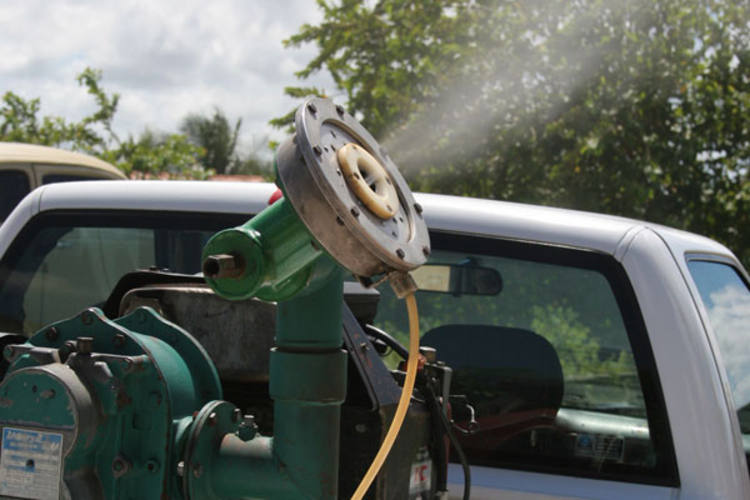
\includegraphics[scale=0.4]{fumace.jpg}
    \caption{Nebulizer equipment attached to vehicle. }
    \label{fig:nebulizer}
\end{figure}

Nebulizer attached to vehicles are very  useful for the control of outbreaks and
epidemics, due to its high performance (80 to 160 blocks per day), however it is
not recommended  in transmission  block situations.  These applications  must be
constantly  supervised to  guarantee the  indicated insecticide  dosage in  each
visited  block, since  there is  a series  of operational  factors, such  as the
equipment flow,  and vehicle speed \citep{brasil-dept-helth:2009}.  In order for
the applications  to have the  desired effectiveness, it  must be realized  in a
period with correct conditions to maintain the insecticide cloud moving close to
the ground.  The thermal inversion is  generally produced in the  morning, after
the sunrise, and in the afternoon, just before sunset, these moments are optimal
to apply the insecticide with the nebulizer vehicle.

The  nebulized insecticide  doesn't  have  residual effect  and  it is  strongly
influenced  by  wind.  The  best  results  are  achieved  when  the  most  dense
insecticide cloud is  at a distance of  up to 100 meters from  the equipment. As
this  distance is  crossed, the  effectiveness  decreases, as  a consequence  of
droplet drift influenced  by factor of the environment. The  cloud dispersion is
illustrated in Figure \ref{fig:dispersion}.

\begin{figure}[!ht]
  \centering
  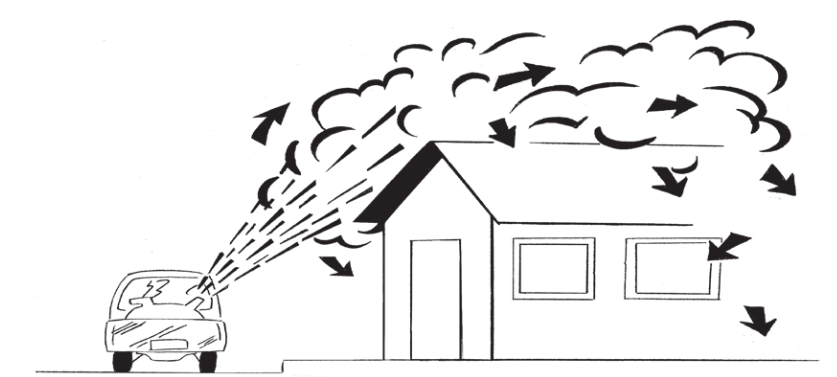
\includegraphics[scale=0.4]{cloud-dispersion.png}
  \caption{Cloud dispersion of the application.}
  \label{fig:dispersion}
\end{figure}

The instructions about the insecticide application method are generally based on
the  ideal conditions  of topology,  structure  of the  locality, and  favorable
winds. The  operation is often harmed  by unpaved roads, presence  of walls, and
high  vegetation,  in  additions  to   headwinds.  Such  this,  the  application
methodology must  consider these limitations  in order  to obtain a  good impact
over the  vector population. The  vehicle must  travel around each  block before
starting the next one, as show in Figure \ref{fig:travel-pattern}.

\begin{figure}[!ht]
  \centering
  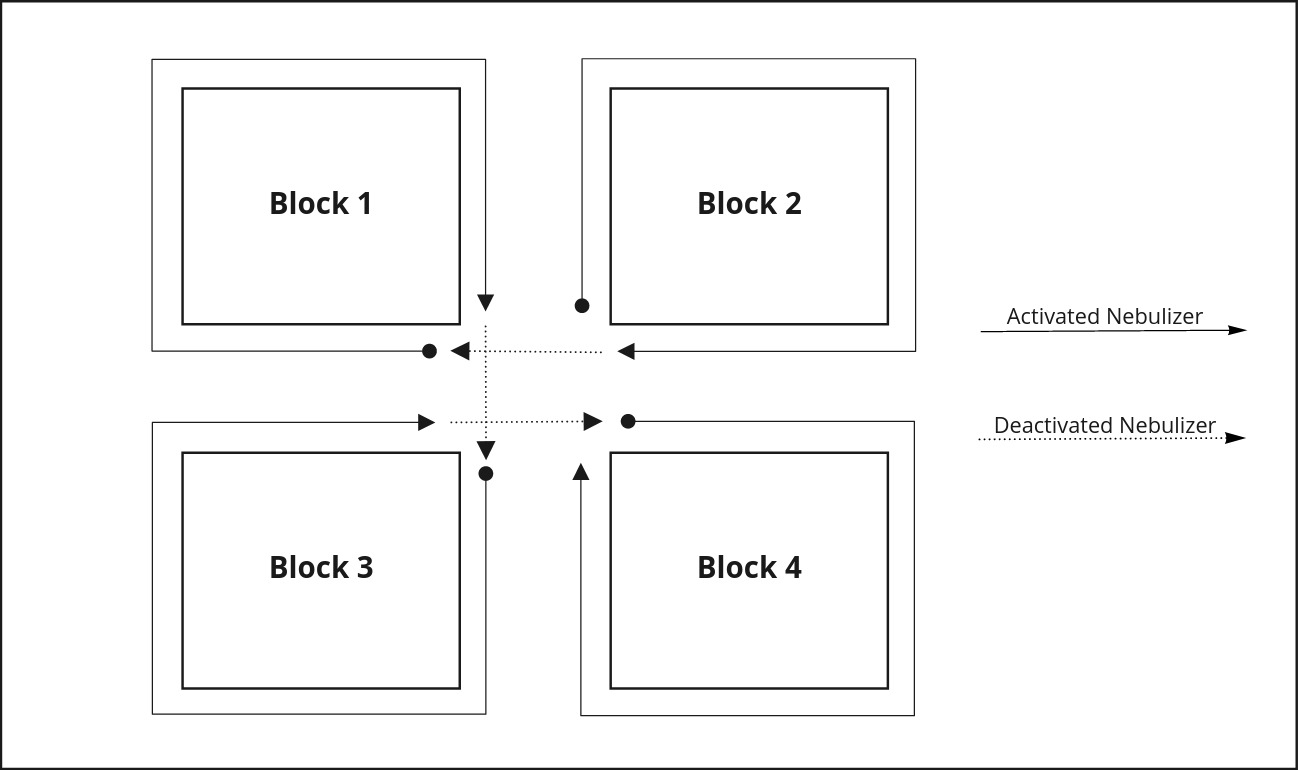
\includegraphics[scale=0.25]{visit-pattern.jpg}
  \caption{Vehicle pattern with nebulizer.}
  \label{fig:travel-pattern}
\end{figure}


The complexity of the process of prevention and control of the disease is large,
involving  only  in  Brazil,  annual   expenses  exceeding  R$\$$  1.6  billions
\citep{negreiros-2020}.  Such  resources could  be  better  used if  the  dengue
logistics was more  effective, and use the resources of  operations research. To
the best of our knowledge, we are  the first to introduce the \gls{dparp}, which
is the problem of  create routes to the nebulizer vehicles  as a \gls{parp} with
resource constraints. \gls{parp}s are arc routing problems where, in addition to
the cost functions, there  is a profit function that must  be taken into account
when an  arc is serviced  \citep{araoz:2006}. In  \gls{dparp}, each block  has a
profit value that is related to the number of dengue cases, it is considered the
block-vist pattern described in Figure \ref{fig:travel-pattern}, and we consider
time and insecticide limitations. The goal of the \gls{dparp} is to maximize the
profit  in  order  to nebulizer  a  region.  In  this  work, we  formulated  the
\gls{dparp} using \gls{ilp}.

This work is  organized as follows. In  the next section we present  a review of
the literature ...


\section{Related Work} \label{sec:related-work}

An extensive number  of works in the  literature use \gls{ml} in  the context of
dengue~\citep{shakurat:2015,shakil:2015,hair:2019,sarma:2020,appice:2020}. Some
of  the main  problems  addressed are  generate dengue  diagnoses  based on  the
patient's symptoms  and clinical patterns,  distinguish dengue and its  types in
the early stage of disease progression  and, dengue fever predictions in certain
regions  based on  a  set of  factors, such  as  precipitation, rain,  humidity,
temperature, and others.

\cite{lowe:2015} presented a  modeling procedure to quantify the  added value of
including  climate  information in  a  dengue  model  for  the 76  provinces  of
Thailand,  from  1982-2013  providing  decision  support  systems.  The  authors
considered a set  factors that have a statistically  significant contribution to
the relative  risk of  dengue in  the following months.  The system  provided an
advanced warning that enable the implementation of a more effective surveillance
system.  According  to  the  authors,  the model  framework  presented  here  is
extremely flexible and could be  applied in any geographical setting, generating
a  more global  approach  to assessing  the impact  of  climate variability  and
climate change on dengue risk.

\cite{bannwart-sbpo:2013,bannwart:2013}   proposed   numeric  techniques   using
genetic  algorithm  to solve  the  control  model  applied  to the  problems  of
combating dengue,  in which the  goal is to minimizes  the cost of  the chemical
control  (insecticide) and  genetic  (liberating sterile  males  in the  natural
environment). These works  assumes that the mortality rate of  the mosquitoes is
strongly  related  to the  investment  in  control approaches.  The  experiments
considered a time period  of 120 days and the results  indicated that the amount
of insecticide used was high considering the other approaches cited in the work,
however  the authors  presented an  analysis  considering each  control and  the
impact on the rate of reduction in the mosquito population.

\cite{cantane:2015} presented an experiment to  obtain the estimate rate used in
a  mathematical  model. The  mosquito  population  was conducted  under  optimal
conditions, simulating favorably  environment for its grow. Life  cycle data was
collected  daily, and  all  estimated  rates used  in  the  equation system  are
computed. It is  notorious that, without a control action,  the population could
highly  increase in  a short  amount  of time.  The results  of the  experiments
provide estimates of  the life cycle of the mosquitoes  are in perfect condition
in nature and the model allows to  measure a approximate number of mosquitoes in
the nature for this scenario.

\cite{dosreis:2018,florentino:2018,florentino-b:2018}   presented   a   set   of
methodologies for dengue control, such  as mathematical model that describes the
population dynamics of the Aedes aegypti, and designed a generic control law for
the mosquito population through  exact linearization techniques. Some heuristics
such as Genetic Algorithm (GA) in which the main goal is to establishing optimal
strategies using  an integration of  different types  of control and  a Variable
Neighborhood Search  (VNS) that determine  optimized control strategies  for the
aquatic phase, producing a lower cost control to reduce the mosquito population.
Some advantages  presented are  that the  control in  aquatic phase  reduces the
environment impact and the need for chemical control in large scale. The results
obtained by computer simulations indicated  that the presented methodologies has
great potential as a tool for support decision maker against arboviroses.

The works of \cite{negreiros:2008,negreiros:2011,negreiros-2020}, to the best of
our knowledge, are the only papers that apply operations research techniques for
the context  of routing  problem along  with the  mosquito control.  These works
focuses on the computational tool called Web Dengue, aimed at helping the dengue
control managers providing  a better visualization of the  problem dimension and
better coordination of control procedures.  Among the methodologies presented in
\cite{negreiros:2008,negreiros:2011},   the   authors    developed   a   integer
programming  formulation  to compute  a  periodical  scheduling of  vehicles  in
determined areas. Also, in \cite{negreiros:2011} was developed a GRASP heuristic
to create routes for the vehicles with nebulizer, and the proposed algorithm was
applied  in a  instance  corresponding  to the  location  of  Praia de  Iracema,
Fortaleza.

\section{Mathematical Formulation for Dengue-PARP} \label{sec:formulation}

Consider a weighted, connected, and directed graph $G = (V, E)$, being $V = \{1,
\dots, n\}$ the  set of $n$ vertices, $E =  \{(i, j): i \text{ and }  j \in V, i
\neq j\}$ the set of $m$ edges. A block, in the \gls{dparp}, can be defined as a
cycle $c$ such that the edges $(i, j) \in C$ are in clockwise order. The set $B$
contains all  blocks of the instance,  and each vertex  $i \in V$ belongs  to at
least one  block, while each  edge $(i, j)  \in E$ is in  at most one  block. In
order to allows the  route starts and end in any vertex of  $G$, it is necessary
to change  $V$ to $V'$ by  adding an artificial  source vertex $s$ and  a target
$t$. It is  also necessary add a set of  edges such that $E' = E  \cup \{(s, u),
(u, t)\} \forall u in V$.

Each edge of $G$ contains two associated values: number of notified dengue cases
and distance in meters.  We set the \gls{dparp} entry as a  tuple ($G(V, E'), s,
t, B, \lambda, \xi, f^T, f^I, \Delta_i, \Delta_t$), where each edge contains the
values of  dengue cases ($\lambda$),  and distance ($\xi$). Consider  a function
$f^T$ that,  with some  notation abuse,  compute the  time to  travel in  a edge
($f^T_{(i, j)}$) and the  time to visit all the edges of  a block ($f^T_b$). The
function $f^I_b$  compute the amount of  insecticide used in a  nebulized block.
Lastly, consider the  maximum amount of insecticide  available ($\Delta_i$), and
the maximum time of the route ($\Delta_t$).

The computed  route can ignore the  cycles that make up  a block, i. e.,  if the
model consider a block as nebulized the  route must contains at least one vertex
from  the block  visited by  the  route. This  approach takes  advantage of  the
nebulizer pulverization pattern presented for  this problem, that must cover all
the  edger  before   move  to  nebulize  another  block.  Next,   we  present  a
single-vehicle \gls{ilp} formulation for the \gls{dparp}.

\subsection{Single-vehicle ILP formulation}

\begin{align}
  \nonumber x_{ij} = & \begin{cases}
                         1, & \text{If the arc $(i, j)$ belongs to the route,} \\
                         0, & \text{CC} 
                       \end{cases} & \forall (i, j) \in E'. \\
  \nonumber y_{ib} = & \begin{cases}
                         1, & \text{If the vertex $i$ are used as start to nebulize the block $b$,} \\
                         0, & \text{CC} 
                       \end{cases} & \forall i \in V', b \in B.
\end{align}


\begin{align}
  \max & \sum_{i \in V'} \sum_{b \in B} \lambda_b y_{ib} - \sum_{ij \in E'} x_{ij} & \label{eq:of}\\
       & \sum_{j \in V'\backslash \{t\}} x_{sj} = 1, & \label{eq:s-all} \\
       & \sum_{j \in V'\backslash \{s\}} x_{jt} = 1, & \label{eq:all-t} \\
       & \sum_{j: (i, j) \in E'} x_{ji} - \sum_{j: (i, j) \in E'} x_{ij} = 0, & \ \forall i \in V' \backslash \{s, t\} \label{eq:flow-conservation} \\
       % & \sum_{(i, j) \in (S, \bar{S})} x_{ij} \geq y_{ib}, & \ \forall S \subset V, i \in S, b \in B(i) \\
       & \sum_{(i, j) \in A'} f^T_{ij} x_{ij} + \sum_{i \in V} \sum_{b \in B} f^T_b y_{ib} \leq T_{\max}, & \\
       & \sum_{i \in V'} \sum_{b \in B} f^I_b y_{ib} \leq I_{\max}, & \\
       & \sum_{i \in V(b)} y_{ib} \leq 1, & \ \forall b \in B, \\
       & \sum_{(i, j) \in A'} x_{ji} \geq y_{ib}, & \ \forall i \in V(b), b \in B.
\end{align}


\begin{itemize}
\item Schedule: 2 horas before or after the sunrise and 2 hours before or after the sundown. Total of 8 hours per day;
\item A minimum geometric distance of 150 meters (radius) from the notified case; 
\item Grouping the cases of a area, preferably for a period of two weeks. Considering the probable life expectancy of the infected adult female;
\item 3 or 5 applications cycle in the same area, each cycle with three or five days. If necessary, the application can be carried out for two more cycles;
\item The recommended velocity of the vehicle is 15km/h, but adjusting the flow of the nebulizer, the velocity can variate from 10km/h to 16km/h;
\item Normal block 400m, 100m for each street;
\item The insecticide must be made on the day of application, or up to 24 hours
  before.
\end{itemize}

\section{Submiss\~ao do Texto Completo}

Ap\'os cadastrar o artigo, o autor \'e convidado a carregar para o sistema de submiss\~ao um arquivo 
de termina\-\c c\~ao DOC ou PDF, com o texto completo. 
A primeira p\'agina desse manuscrito deve conter o t\'itulo do artigo coincidindo exatamente com o informado quando do cadastramento. 
Deve, tamb\'em, incluir novamente os resumos e palavras-chave em portugu\^es ou espanhol e ingl\^es, e o(s) t\'opico(s) organizado(s) 
em ordem de prioridade, mas \textbf{n\~ao pode incluir nomes de autores}.

Este manuscrito ser\'a disponibilizado para o exame pelos revisores, que ter\~ao tamb\'em acesso
 \`as informa\c c\~oes do cadastro, exceto as referentes aos nomes e institui\c c\~oes dos autores. 
Uma vez aceito o artigo, os autores ser\~ao chamados a encaminhar \textbf{vers\~ao final} com a p\'agina inicial completa, isto \'e, com autores, institui\c c\~oes, resumo de no m\'aximo 150 palavras, 3 palavras-chave, t\'opicos, \textit{abstract}, \textit{keywords} e \textit{paper topics} .

As p\'aginas deste texto n\~ao devem vir numeradas, tanto no caso de arquivo enviado quando da submiss\~ao quanto no caso do arquivo com a vers\~ao final do artigo aceito. 
A numera\c c\~ao ser\'a feita posteriormente para o conjunto de todos os artigos.
\textbf{Cabe\c calhos e rodap\'es devem ser deixados em branco}.


\section{ Instru\c c\~oes de Formata\c c\~ao}


Os trabalhos completos devem ter \textbf{no m\'aximo 12 p\'aginas}, inclu\'idos neste limite: a primeira p\'agina com resumo, texto, tabelas, gr\'aficos, agradecimentos e refer\^encias.

Os textos devem utilizar p\'aginas de tamanho \textbf{A4} (29,7 x 21,0 cm) com \textbf{margem superior de 3,3 cm, inferior de 2,5 cm e laterais de 2,9 cm}.
 Devem ser escritos em coluna \'unica, com fonte \textbf{\textit{Times New Roman} 11}. 



\section{ Estilo das Cita\c c\~oes}


As cita\c c\~oes no texto devem estar entre colchetes e conter  os \'ultimos sobrenomes dos autores~\citep{silva:99}, no caso de um ou dois autores, e o \'ultimo sobrenome seguido de "et al." no caso de mais de dois autores, seguidos do \textbf{ano da publica\c c\~ao}, como por exemplo,~\citep{anna:06},~\citep{gates:03}, ~\citep{smith:02}, ~\citep{silva:99}, ~\citep{pele:04}, ~\citep{web:16}.
As refer\^encias no final do texto devem estar em ordem alfab\'etica do \'ultimo sobrenome do primeiro autor. 


~\\
\bibliographystyle{sbpo}
\bibliography{exemplo-latex}


\end{document}

